% !TEX root = ../my-thesis.tex
%
\chapter{The Standard Model of Particle Physics}
\label{sec:sm}

\cleanchapterquote{Tyger, tyger, burning bright \\ In the forests of the night, \\ What immortal hand or eye \\ Could frame thy fearful symmetry?}{William Blake}{Poems of William Blake, edited by W. B. Yeats. London: G. Routledge \& Sons, 1905}


\section{Introduction}
\label{sec:sm:introduction}
The Standard Model of electroweak and strong interactions (SM) is the relativistic quantum field theory, which describes the elementary constituents of matter and their interactions. It is the empirically adequate theory of Nature, as its validity is supported by a large number of measurements, including the observation of the weak gauge bosons~\cite{Arnison1983,Banner1983,Arnison1983-2,Bagnaia1983}, the discovery of the top quark~\cite{Abachi1995,Abe1995}, and the discovery of the Higgs boson~\cite{HIGG-2012-27,CMS-HIG-12-028}.

The constituents of matter are the particles with half-integer spin, which are called fermions. All known interactions between the particles in the SM are dictated by the underlying internal symmetries of the theory. The gauge principle naturally introduces the spin-1 gauge bosons as mediators of forces by insisting on the invariance of the theory under local phase transformations. Interactions between particles are described by the exchange of gauge bosons. The masses of the fermions and massive gauge bosons are generated in a gauge-invariant way by Yukawa-interactions and electroweak spontaneous symmetry breaking. The spin-0 Higgs boson is a direct consequence of the latter mechanism.

This chapter gives a brief introduction to the salient concepts of the SM, following the presentation in Refs.~\cite{Hollik2010,Halzen1984} closely. A more complete and pedagogic treatment is given in Refs.~\cite{Maggiore2005,Peskin1995,Schwartz2013}.

\newpage

\section{The Standard Model gauge group}
\label{sec:sm:gauge}
The SM is a Yang-Mills theory~\cite{Yang1954,tHooft1972} based on the gauge group
\begin{align}
    \textrm{SU}(3)_{C} \times \mathrm{SU}(2)_{L} \times \mathrm{U}(1)_{Y}.
\end{align}
\begin{itemize}
    \item The \(\textrm{SU}(3)_{C}\) component is the colour symmetry group associated with the \textbf{strong interaction}, which is described by quantum chromodynamics (QCD)~\cite{Gross1973,Gross1973-2,Politzer1973,Fritzsch1973}. All particles carrying colour charge participate in the strong interaction. The gauge bosons of  strong interactions are the eight massless gluons \(G_{\mu}^{a}, a=1, \dots, 8\), which themselves also carry colour charge. The coupling constant of the strong interaction is \(g_{s}\), or equivalently \(\alpha_{s} = g_{s}^2 / 4 \pi\).

    \item The \(\mathrm{SU}(2)_{L} \times \mathrm{U}(1)_{Y}\) component is the symmetry group associated with \textbf{electroweak interactions}~\cite{Glashow1961,Weinberg1967,Salam1994}. All particles carrying weak isospin \((I, I_{3})\) and weak hypercharge \(Y\) participate in electroweak interactions. The gauge bosons \(W^{i}_{\mu}\), \(i=1, 2, 3\), and \(B_{\mu}\), and the gauge coupling constants \(g\) and \(g'\) correspond to the factors \(\mathrm{SU}(2)_{L} \times \mathrm{U}(1)_{Y}\), respectively. The electroweak symmetry has to be broken by the Brout-Englert-Guralnik-Hagen-Higgs-Kibble mechanism~\cite{Englert1964,Higgs1964,Higgs1964-2,Guralnik1964,Higgs1966,Kibble1967} to describe the massive \PWpm, \PZ gauge bosons of the weak interaction and unveil the electromagnetic \(\textrm{U}(1)_{Q}\) gauge symmetry. The quantum numbers classifying the fermions with respect to the \(\mathrm{SU}(2)_{L} \times \mathrm{U}(1)_{Y}\) group and their electric charge \(Q\) are related by the Gell-Mann-Nishijima relation \(Q = I_{3} + Y / 2\)~\cite{Nakano1953,GellMann1956}.

    Only the left-handed chirality eigenstates of the fermions
    \begin{align}
        \psi(x)_{L} = \frac{1}{2}(1 - \gamma_{5}) \psi(x)
    \end{align}
    carry weak isospin \(I_{3} = \pm \nicefrac{1}{2}\) and can participate in flavour-changing interactions via couplings to the charged \PWpm bosons.

    The right-handed chirality eigenstates of the fermions
    \begin{align}
        \psi(x)_{R} = \frac{1}{2}(1 + \gamma_{5}) \psi(x)
    \end{align}
    carry weak isospin \(I_{3} = 0\) and do not couple to the weak gauge bosons, leading to maximum parity violation in the weak interaction.
\end{itemize}

\section{Particle content of the Standard Model}
\label{sec:sm:particles}
The fermions are categorised in quarks and leptons. \Cref{fig:sm:fermions} shows a schematic overview of the quarks and leptons arranged in three different generations. The three generations appear to have identical gauge interactions and only differ by their flavour quantum number and their mass. To every fermion, there is a corresponding anti-fermion with the same mass and spin but inverted charge quantum numbers (not shown in \Cref{fig:sm:fermions}).
\begin{figure}[htbp]
	\centering
	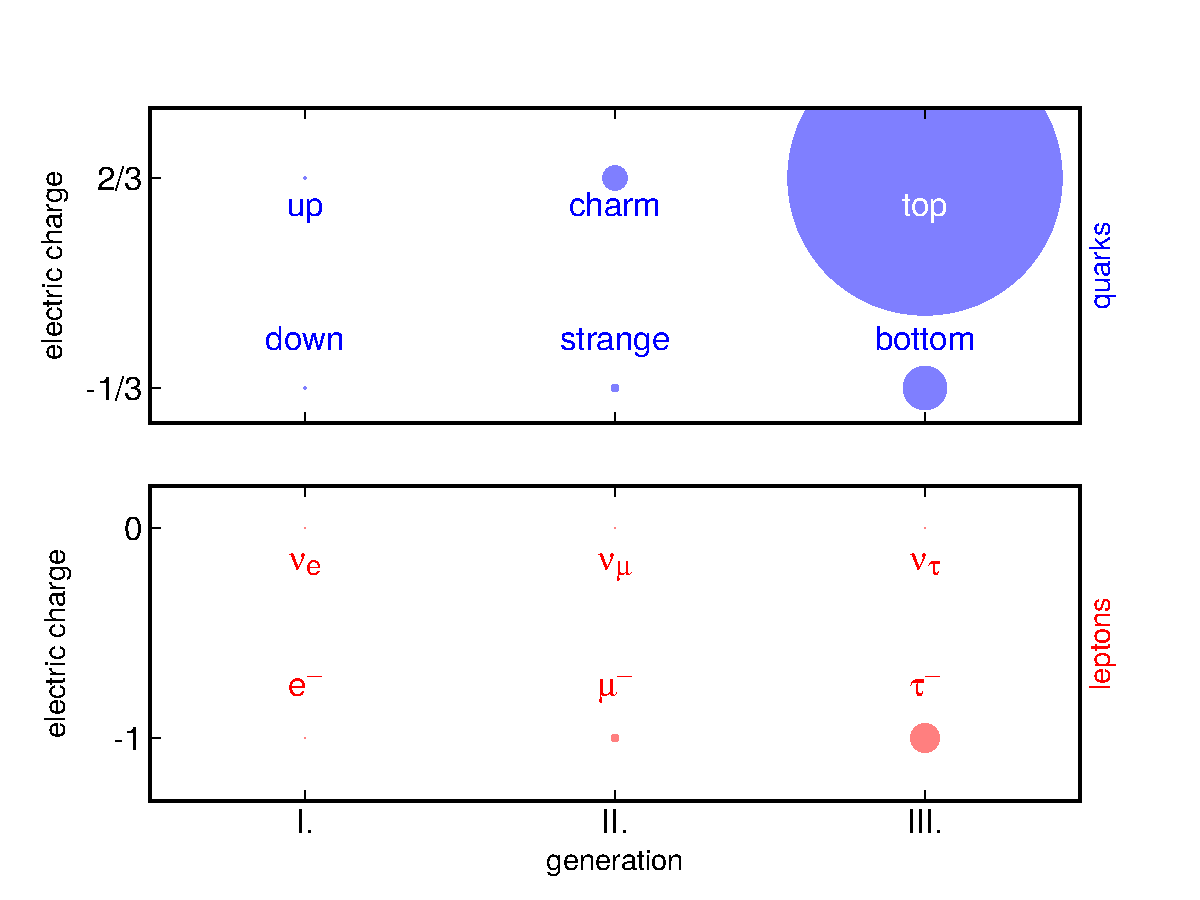
\includegraphics[width=0.95\textwidth]{figures/standardmodel/sm_fermions.pdf}
	\caption{Schematic overview of quarks and leptons, grouped by affiliation to generation and electric charge. The size of the circles is proportional to the fermion mass.}
	\label{fig:sm:fermions}
\end{figure}

There are six quark flavours, which can be grouped by their electric charge in the up-type quarks \(\Pqu_{i}\) (\(i=1, 2, 3\)) with electric charge \(\nicefrac{2}{3}\) and down-type quarks \(\Pqd_{i}\) (\(i=1, 2, 3\)) with electric charge \(\nicefrac{-1}{3}\). The up-type quarks are the up (\Pqu), charm (\Pqc), and top (\Pqt) quarks. The down-type quarks are the down (\Pqd), strange (\Pqs), and bottom (\Pqb) quarks. Quarks are the only fermions with colour charge \(q^{\alpha}, \alpha=r, g, b\), and are represented as colour charge triplets under \(\textrm{SU}(3)_{C}\)
\begin{align}
    \Pq = \begin{pmatrix} \Pq^{r} \\ \Pq^{g} \\ \Pq^{b} \end{pmatrix}.
\end{align}
The left-handed quarks carry weak isospin \(I_{3} = \pm \nicefrac{1}{2}\) and transform as doublets of up- and down-type quarks under \(\mathrm{SU}(2)_{L}\)
\begin{align}
    \begin{pmatrix} \Pqu \\ \Pqd' \end{pmatrix}_{L}, \begin{pmatrix} \Pqc \\ \Pqs' \end{pmatrix}_{L}, \begin{pmatrix} \Pqt \\ \Pqb' \end{pmatrix}_{L},
\end{align}
whereas the right-handed quarks carry weak isospin \(I_{3} = 0\) and transform as singlets
\begin{align}
\Pqu_{R}, \Pqd_{R}, \Pqc_{R}, \Pqs_{R}, \Pqt_{R}, \Pqb_{R}.
\end{align}
Here, \(\Pqd'_{i} = \Pqd', \Pqs', \Pqb'\) are the weak eigenstates, which are obtained from of the mass eigenstates \(\Pqd_{i} = \Pqd, \Pqs, \Pqb\) by a rotation \(\Pqd'_{i} = \sum_{j} V_{ij} d_{j}\) with the Cabibbo-Kobayashi-Maskawa mixing matrix~\cite{Cabibbo1963,Kobayashi1973,Tanabashi2018}
\begin{align}
\begin{split}
    V &= \begin{pmatrix} %
    	\Vud & \Vus & \Vub \\%
    	\Vcd & \Vcs & \Vcb \\%
    	\Vtd & \Vts & \Vtb%
    \end{pmatrix} \\
       &=  %
    \begin{pmatrix}%
    	\num{0.97417} \pm \num{0.00021} & \num{0.2248} \pm \num{0.0006} & \num{0.000409} \pm \num{0.000039} \\%
    	\num{0.220} \pm\num{0.005} & \num{0.995} \pm \num{0.016} & \num{0.00405} \pm \num{0.0015} \\%
    	\num{0.0082} \pm \num{0.0006} & \num{0.04} \pm \num{0.0027} & \num{1.0009} \pm \num{0.031}%
    \end{pmatrix}.
\end{split}
\end{align}
Quarks participate in strong, electromagnetic, and weak interactions.

There are six lepton flavours, which also can be grouped by their electric charge in the charged leptons and neutral leptons. The charged leptons are the electron (\Pem), the muon (\Pgmm), and the tau lepton (\Pgtm). They carry the electromagnetic charge \(q_{\Plpm_{i}} = - 1\). The neutral leptons are the associated neutrinos \Pgne, \Pgngm, \Pgngt.
The left-handed leptons carry weak isospin \(I_{3} = \pm \nicefrac{1}{2}\) and transform as doublets under \(\mathrm{SU}(2)_{L}\)
\begin{align}
\begin{pmatrix} \Pgne \\ \Pem \end{pmatrix}_{L}, \begin{pmatrix} \Pgngm \\ \Pgmm \end{pmatrix}_{L}, \begin{pmatrix} \Pgngt \\ \Pgtm \end{pmatrix}_{L},
\end{align}
whereas the charged right-handed leptons carry weak isospin \(I_{3} = 0\) and transform as singlets
\begin{align}
\Pem_{R}, \Pgmm_{R}, \Pgtm_{R}.
\end{align}
To date, neither right-handed neutrinos nor left-handed anti-neutrinos have been observed. The charged leptons participate in electromagnetic and weak interactions, while the neutrinos only participate in weak interactions.


\section{The Standard Model in the Lagrangian formalism}
\label{sec:sm:lagrangian}
The SM is elegantly and concisely formulated in the Lagrangian formalism of quantum field theory. The particles are described by quantum fields, which are operators on the Hilbert space of particle states. The fermions are described by spin-\(\nicefrac{1}{2}\) spinor fields \(\psi(x)\). The gauge bosons are described by spin-1 vector fields \(A_{\mu}\). The Higgs boson, the only spin-\(0\) particle in the SM, is described by a scalar field \(\phi(x)\).

Remarkably, all dynamics of elementary particles are determined by the action
\begin{align}
    S[\varphi] = \int \dd{x} \mathcal{L}\left(\varphi(x), \partial_{\mu}\varphi(x)\right),
\end{align}
where \(\varphi\) is a generic field variable and \(\mathcal{L}\left(\varphi(x)\right)\) is the Lorentz-invariant Lagrangian (density). The equations of motions for elementary particles are obtained by the means of Hamilton's principle
\begin{align}
    \delta S = S[\varphi + \delta \varphi] - S[\varphi] = 0.
\end{align}

The Lagrangian of the SM consists of the four parts\footnote{In principle, \(\mathcal{L}\), could be extended by a term associated with the strong interaction, violating charge and parity (CP) symmetry. As there is no evidence for CP violation in strong interactions, this term is neglected. Also, additional gauge-fixing terms, e.g. \(\delta \mathcal{L} = - (\partial_{\mu} A^{\mu})^2 / 2 \zeta\) with the parameter \(\zeta\) for a gauge field \(A_{\mu}\), are neglected in the following discussion.}
\begin{align}
    \mathcal{L} = \mathcal{L}_{\text{Gauge}} + \mathcal{L}_{\text{Fermion}} + \mathcal{L}_{\text{Higgs}} + \mathcal{L}_{\text{Yukawa}},
\end{align}
which are described in the following paragraphs.

\subsection{Gauge boson kinetic term}
\label{sec:sm:lagrangian:boson}
The gauge-invariant gauge boson kinetic term
\begin{align}
    \mathcal{L}_{\text{Gauge}} = - \frac{1}{4} G_{\mu\nu}^{a} G^{\mu\nu}_{a} - \frac{1}{4} W^{i}_{\mu\nu} W_{i}^{\mu\nu} - \frac{1}{4} B_{\mu\nu} B^{\mu\nu}
\end{align}
is required to promote the gauge bosons, which emerge from the gauge principle, to dynamical fields. It consists of the field strength tensors of the strong interaction
\begin{align}
    G_{\mu\nu}^{a} = \partial_{\mu} G_{\nu}^{a} - \partial_{\nu}G_{\mu}^{a} - g_s f_{abc} G_{\mu}^{b} G_{\nu}^{c},
\end{align}
where \(f_{abc}\) denotes the structure constants of the \(\textrm{SU}(3)_{C}\) group, and the field strength tensors for the electroweak gauge bosons
\begin{align}
    W^{i}_{\mu\nu} &= \partial_{\mu} W_{\nu}^{i} - \partial_{\nu} W_{\mu}^{i} + g W_{\mu}^a,
\end{align}
where the totally antisymmetric tensor \(\varepsilon_{ijk}\) denotes the structure constants of the \(\textrm{SU}(2)_{L}\) group. The terms associated with the structure constants are responsible for the non-trivial gauge transformations and introduce the three- and four-point direct interactions among the weak gauge bosons and among the gluons. No explicit mass terms are present in \(\mathcal{L}_{\text{Gauge}}\), as their presence would violate gauge invariance. They are introduced via electroweak spontaneous symmetry breaking.

\subsection{Fermion kinetic and interaction term}
\label{sec:sm:lagrangian:fermion}
The fermion kinetic term introducing interactions with the gauge bosons
\begin{align}
    \mathcal{L}_{\text{Fermion}} = \sum_{j} \overline{\psi}_{L}^{j} i \gamma^{\mu} D_{\mu}^{L} \psi_{L}^{j} + \sum_{j, \sigma} \overline{\psi}_{R\sigma}^{j} i \gamma^{\mu} D^{R}_{\mu} \psi^{j}_{R\sigma}
\end{align}
describes the left-handed fermion fields \(\psi_{L}^{j, T} = (\psi_{L+}^{j} \psi_{L-}^{j})\) and the right-handed fermion fields \(\psi_{R}^{j\sigma}\). They carry the generation index \(j\) and the component index \(\sigma=\pm\), which denotes up-type fermions (\(+\)) and down-type fermions (\(-\)). Their interactions with the gauge bosons via the minimal substitution rule is introduced by the covariant derivative
\begin{align}
    D^{L, R}_{\mu} = \partial_{\mu}  - i g_{s} T_{a} G^{a}_{\mu} - i g I^{L,R}_{j} W^{j}_{\mu} + i g' \frac{Y}{2} B_{\mu}.
\end{align}
\(T_{a}\), \(I^{L}_{a}\), and \(\frac{Y}{2}\) are the generators of the groups \(\textrm{SU}(3)_{C}\), \(\textrm{SU}(2)_{L}\), and \(\textrm{U}(1)_{Y}\), respectively. They are defined by \([T_{a}, T_{b}] = i f_{abc} T_{c}\) and \([I^{L}_{a}, I^{L}_{b}] = i \varepsilon_{abc} I^{L}_{c}\). In the triplet representation, \(T_{a} = \frac{1}{2} \lambda_{a}\) can be written with the Gell-Mann matrices \(\lambda_{a}, a=1, \dots, 8\). Similarly, \(I_{j}^{L} = \frac{1}{2} \sigma_{j}\) can be written in the doublet representation with the Pauli matrices \(\sigma_{j}, j=1,2,3\). For the sake of consistent notation, the associated term for right-handed particles is \(I_{j}^{R} = 0\).
No mass terms for Fermions are included in \(\mathcal{L}_{\text{Fermion}}\), as they would mix left- and right-handed fields and would explicitly break gauge invariance. The fermion mass terms are introduced via gauge-invariant Yukawa interactions between the fermions and the Higgs field.

\subsection{The Higgs mechanism in the Standard Model}
\label{sec:sm:lagrangian:higgs}
The Higgs field term
\begin{align}
    \mathcal{L}_{\textrm{Higgs}} = (D_{\mu} \phi)^{\dag} (D^{\mu} \phi) - V(\phi)
\end{align}
introduces a complex scalar Higgs doublet \(\Pphi = \begin{pmatrix} \Pphi^{+} \\ \Pphi^{0} \end{pmatrix}\) with hypercharge \(Y=1\) and the covariant derivative
\begin{align}
    D_{\mu} = \partial_{\mu} + i g \frac{1}{2} \sigma_{j} W_{\mu}^{j} + i g' \frac{Y}{2} B_{\mu}.
\end{align}
The Higgs potential
\begin{align}
    V(\Pphi) = \mu^2 \Pphi^{\dag} \Pphi + \frac{\lambda}{4} (\Pphi^{\dag} \Pphi)^2.
\end{align}
has two free parameters \(\mu^2\) and \(\lambda > 0\). For \(\mu^2 > 0\), \(\mathcal{L}_{\textrm{Higgs}}\) describes a scalar field with mass \(\mu\) which can self-interact via a four-point interaction vertex with coupling \(\lambda\) and whose ground state corresponds to \(\phi = 0\). More interesting is the case \(\mu^2 < 0\), which is shown in \Cref{fig:sm:higgs-potential} for a specific choice of these parameters, as it allows introducing mass terms for the gauge bosons via spontaneous symmetry breaking while respecting the \(\text{SU}(2)_{L} \times \textrm{U}(1)_{Y}\) gauge-invariance.
\begin{figure}[htbp]
    \centering
    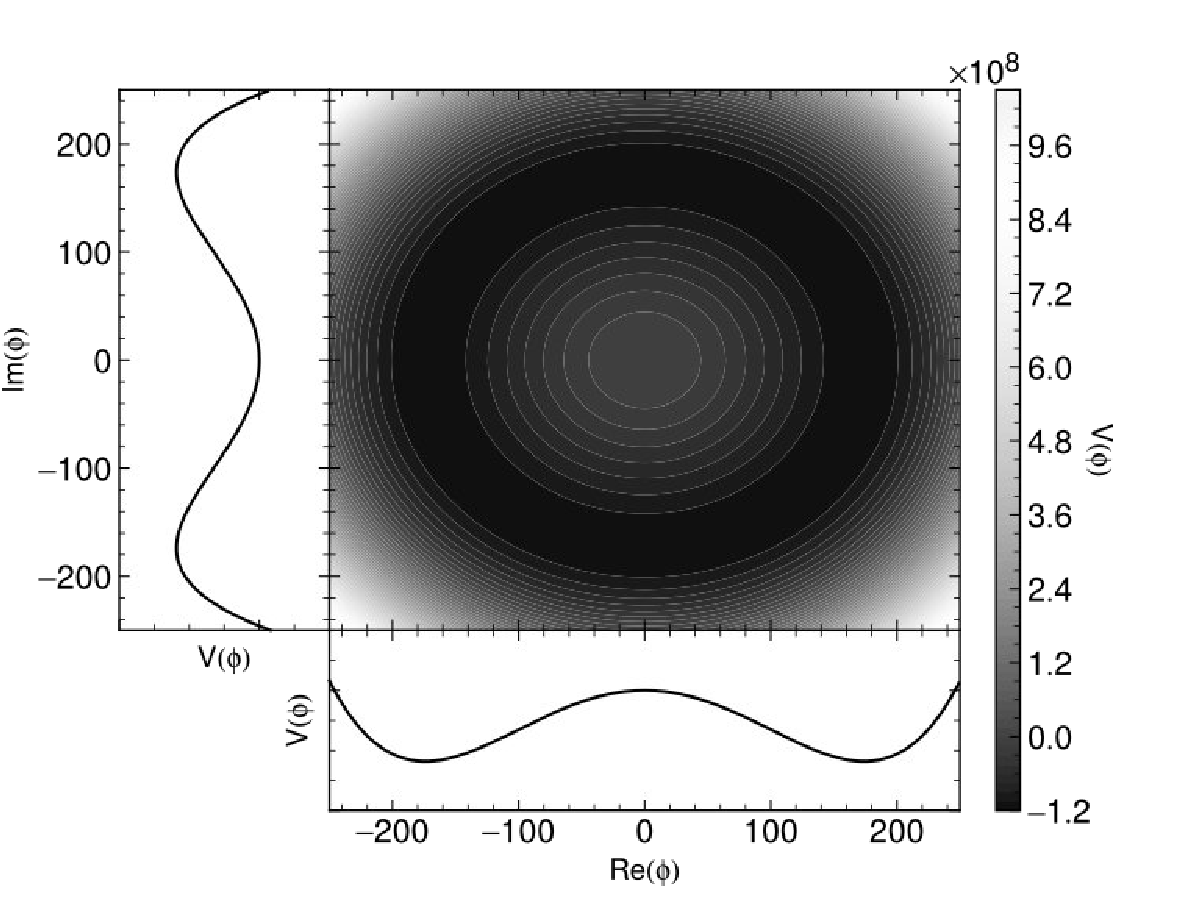
\includegraphics[width=0.95\textwidth]{figures/standardmodel/sm_higgs_sw.pdf}
    \caption{The Higgs potential \(V(\phi)\) with parameters \(\mu^2 = -(\SI{125}{\giga\electronvolt})^2 / 2\) and \(\lambda = 0.13\) is shown in dependency of the real and imaginary part of \(\phi\). For this choice of parameters \(\mu^2 < 0\) and \(\lambda > 0\) the potential assumes its minimum at the circle with radius \(v / \sqrt{2} = \SI{246}{\giga\electronvolt} / \sqrt{2}\), which is defined by the vacuum expectation value \(v\).}
    \label{fig:sm:higgs-potential}
\end{figure}
The potential \(V(\phi)\) is minimised by all field configurations on the circle in the \(\text{Re}(\phi)\)-\(\text{Im}(\phi)\)-plane defined by \(\abs{\phi}^2 = 2 \mu^2 / \lambda\).
Choosing the specific real and electrically neutral ground state configuration
\begin{align}
    \phi_0 = \expval{\phi}{0} = \frac{1}{\sqrt{2}} \begin{pmatrix} 0 \\ v \end{pmatrix},
\end{align} spontaneously breaks the \(\textrm{SU}(2)_{L} \times \textrm{U}(1)_{Y}\) symmetry of the Lagrangian. Here, \(v = 2 \mu / \sqrt{\lambda}\) denotes the vacuum expectation value.
Although the specific choice of the ground state breaks the symmetry, the Lagrangian and the physical system are still invariant under symmetry operations%
    \footnote{This statement can be illustrated by considering a scalar field \(\phi\) and a potential \(V = V(\abs{\phi})\). The potential possesses a \(\textrm{U}(1)\) symmetry and the associated Lagrangian density \(\mathcal{L} = \abs{\partial_{\mu} \phi}^2 - V(\abs{\phi})\) is symmetric under transformations \(\phi \mapsto \phi' = e^{i \alpha} \phi\). If the minimum \(\phi_{0} = v\) of the potential \(V\) does not occur at \(v=0\), the symmetry of the ground state is broken \(\phi_{0}' = e^{i \alpha} v \neq \phi_{0}\).}.

The \(U(1)_{Q}\) symmetry of the vacuum, corresponding to the conservation of electric charge, remains unbroken, as the operator associated with electric charge \(Q = I_3 + \frac{Y}{2}\) leaves the ground state invariant.

Perturbative calculations should involve expansions around the ground state. The Higgs doublet can be expanded around the ground state \(\phi_{0}\) in the real field \(h(x)\) and the three real fields \(\theta^{i}(x)\)
\begin{align}
\phi(x) = \frac{1}{\sqrt{2}} \begin{pmatrix} 0 \\ v + h(x) \end{pmatrix} e^{i I^{L}_{j} \theta^{j}(x)}.
\end{align}
In the unitary gauge, \(\theta^{j}(x) = 0\), the massless Goldstone modes \(\theta^{j}(x)\) are absorbed by the weak gauge bosons, giving them a longitudinal polarisation. The Higgs field term after spontaneous symmetry breaking now reads
\begin{align}
\begin{split}
    \mathcal{L}_{\textrm{Higgs}} = & \frac{1}{2} \partial^{\mu} h \partial_{\mu} h - \mu^2 h^2 \\
    & +  \frac{g^2}{8} v^2 \left(W_{\mu}^{+} W^{\mu +} + W_{\mu}^{-} W^{\mu -} \right) + \frac{g^2}{4 \cos^2 \theta_{W}} v^2 Z_{\mu}Z^{\mu} \\
    & + (2vh + h^2) \left(\frac{g^2}{4} W_{\mu}^{+} W^{\mu -} + \frac{g^2}{8 \cos^2 \theta_{W}} Z_{\mu}Z^{\mu}\right) \\
    & + \lambda v h^3 + \frac{\lambda}{4} h^4.
\end{split}
\label{eq:sm:lagrangian:higgs:broken}
\end{align}
It explicitly describes (with the number corresponding to the line in \Cref{eq:sm:lagrangian:higgs:broken})
\begin{enumerate}
    \item the massive real scalar Higgs boson with explicit kinetic and mass term,
    \item the mass terms \(m_{\PWpm} = g^2 v^2 / 4\) and \(m_{\PZ} = g^2 / 8 \cos^2 \theta_{W}\) for the massive weak vector gauge bosons \PWpm and \PZ, respectively,
    \item interactions between the Higgs boson and the weak vector gauge bosons, and
    \item triple and quartic couplings of the Higgs boson.
\end{enumerate}

After electroweak symmetry breaking the associated four gauge fields are
\begin{align}
    W^{\pm}_{\mu} &= \frac{1}{\sqrt{2}} \left(W^{1}_{\mu} \pm W^{2}_{\mu} \right), \\
    Z_{\mu} &= W_{\mu} \cos \theta_{W} - B_{\mu} \sin \theta_{W} \\
    A_{\mu} &= B_{\mu} \cos \theta_{W} + W_{\mu}^{3} \sin \theta_{W}
\end{align}
where \(Z_{\mu}\) and \(W^{\pm}_{\mu}\) are the neutral and charged massive gauge bosons mediating the weak interaction. \(A_{\mu}\) is the photon mediating the electromagnetic interaction. The Weinberg angle \(\theta_{W}\) is defined by the couplings \(g\) and \(g'\) of \(\mathrm{SU}(2)_{L} \times \mathrm{U}(1)_{Y}\)
\begin{align}
    \sin \theta_{W}  = \frac{g'}{\sqrt{g^2 + g'^2}} \quad \cos \theta_{W} = \frac{g}{\sqrt{g^2 + g'^2}}.
\end{align}
The electric charge is related to the couplings \(g\) and \(g'\) and to the Weinberg mixing angle by
\begin{align}
    e = g \sin \theta_{W} = g' \cos \theta_{W}.
\end{align}
The electromagnetic coupling constant is customarily expressed by the fine structure constant \(\alpha_{\text{EM}} = e^2 / 4 \pi\).

\subsection{Yukawa interactions between fermions and the Higgs field}
\label{sec:sm:lagrangian:yukawa}
The Yukawa term in unitary gauge (neglecting flavour mixing in the quark sector)
\begin{align}
    \mathcal{L}_{\text{Yukawa}} = - \sum_{f} m_{f} \overline{\psi}_{f} \psi_{f} - \sum_{f} \frac{m_{f}}{v} \overline{\psi}_{f} \psi_{f} h
\end{align}
contains the mass terms \(m_{f} = y_{f} v / \sqrt{2}\), which relate the individual Yukawa coupling constants \(y_{f}\) to the mass of the charged fermions \(f = \Pqu, \Pqd, \dots, \Pgt\). The interactions between the massive fermions and the Higgs boson occur with coupling constants proportional to the fermion masses.

\section{Phenomenology of the Standard Model}
\label{sec:sm:phenomenology}
The non-Abelian structure of the \(\mathrm{SU}(3)_{C}\) and \(\mathrm{SU}(2)_{L}\) symmetry groups results in distinctive properties of strong and weak interactions. The non-trivial transformations of the strong and weak gauge bosons under their respective symmetry groups allow them to interact directly in three- or four-point interactions.

In particular, the direct coupling of gluons has dramatic implications for the strong interaction, which become apparent in considering the effects of charge screening. As an example, consider an electric probe charge near a charged source. The coupling constant of the electromagnetic interaction increases at small distances to a charged source due to the screening of \HepProcess{\Pep\Pem} pairs of the vacuum. This behaviour is known as ``running coupling''. The coupling constant of the strong interaction shows precisely the opposite behaviour, as the vacuum is not only a polarisable medium due to \HepProcess{\Pq\Paq} pairs but also due to gluon pairs. The gluons spread out the effective colour charge of the quark and counteract the effect from quark pairs. The resulting behaviour of quarks interacting at small length scale (high energy) as nearly free particles is known as \emph{asymptotic freedom} and is essential for turning quantum chromodynamics into a quantitative calculational scheme predicting the interactions at particle colliders.

The second defining feature of the strong interaction is the \emph{colour confinement hypothesis}, stating that only colour-singlet states are observed. As a consequence, no free quarks have been observed to date but only bound states of two or more quarks. These bound states are collectively called \emph{hadrons}, with the \emph{baryons} states \(B\) and the \emph{mesons} states \(M\), which are defined by
\begin{align}
    B &= \frac{1}{\sqrt{6}} \varepsilon^{\alpha \beta \gamma} \ket{q_{\alpha} q_{\beta} q_{\gamma}} \\
    M &= \frac{1}{\sqrt{3}} \delta^{\alpha \beta} \ket{q_{\alpha} \overline{q}_{\beta}}.
\end{align}
Recently, exotics bound states of four~\cite{Aaij2017,Aaij2020} or five quarks~\cite{Aaij2015} have been observed, which are in agreement with the colour confinement hypothesis.
Another consequence of the confinement hypothesis, which strikingly manifests in high-energy hadron collision events, is the formation of jets~\cite{Sterman1977}. Jets are collimated sprays of particles emerging from coloured states in a similar manner as a decelerating electric charge emits photons via Bremsstrahlung. When a quark anti-quark pair is separated, their colour interaction increases due to the ``running coupling'' and squeezes the colour field lines into tube-like regions until the increasing potential energy suffices for the creation of another quark anti-quark pair. The repeated formation of clusters of quarks and gluons forming hadrons is called \emph{hadronisation}.


The free parameters SM are empirically determined with great precision. The discovery of the Higgs boson in 2012~\cite{HIGG-2012-27,CMS-HIG-12-028} concluded the experimental inventory of all SM particles and corroborated the local gauge theory with spontaneous symmetry breaking as the empirically adequate description of fundamental interactions.

% A particular choice of a set of free parameters, which are (in principle) directly accessible by experiment is reported in \Cref{tab:sm:parameters}~\cite{Tanabashi2018}.
% \begin{table}[htb]
% \caption{Empirically determined free parameters of the SM}
% \label{tab:sm:parameters}
% \centering
% \begin{tabular}{l r}
% \toprule
% parameter &  value \\
% \midrule
% fine-structure constant \(\alpha_{\text{EM}}\) & \num{0.0072973525693}\\
% Weinberg mixing angle \(\theta_{W}\) & \num{0.23122}\\
% coupling constant of strong interaction \(\alpha_{s}\) & \num{0.1182}\\
% Higgs potential vacuum expectation value \(v\) & \SI{246}{\giga\electronvolt}\\
% Higgs boson mass & \SI{125}{\giga\electronvolt}\\
% up quark mass \(m_{\Pqu}\) & \SI{2.2}{\mega\electronvolt} \\
% down quark mass \(m_{\Pqd}\) & \SI{4.7}{\mega\electronvolt} \\
% strange quark mass \(m_{\Pqs}\) & \SI{96}{\mega\electronvolt}\\
% charm quark mass \(m_{\Pqc}\) & \SI{1.27}{\giga\electronvolt}\\
% bottom quark mass \(m_{\Pqb}\) & \SI{4.18}{\giga\electronvolt}\\
% top quark mass \(m_{\Pqt}\) & \SI{173.21}{\giga\electronvolt}\\
% electron mass \(m_{\Pem}\) & \SI{0.51}{\mega\electronvolt}\\
% muon mass \(m_{\Pgmm}\) & \SI{105.66}{\mega\electronvolt}\\
% tau lepton mass \(m_{\Pgtm}\) & \SI{1.776}{\giga\electronvolt}\\
% CKM matrix mixing angle \(\theta_1\) & (not discussed) \\
% CKM matrix mixing angle \(\theta_1\) & (not discussed) \\
% CKM matrix mixing angle \(\theta_1\) & (not discussed) \\
% CKM matrix CP-violating phase \(\delta_{13}\) & (not discussed)\\
% possible CP-violating strong-interaction parameter & (not discussed)\\
% \bottomrule
% \end{tabular}
% \end{table}
% Once the free parameters are know, the predictions of the SM can be tested with great precision.

The impressive success of the SM in accurately describing the observations across 15 orders of magnitude is demonstrated in cross-section measurements of SM processes by the ATLAS experiment at the Large Hadron Collider, which is shown in \Cref{fig:sm:atlas-measurement}.

\begin{figure}[htbp]
    \centering
    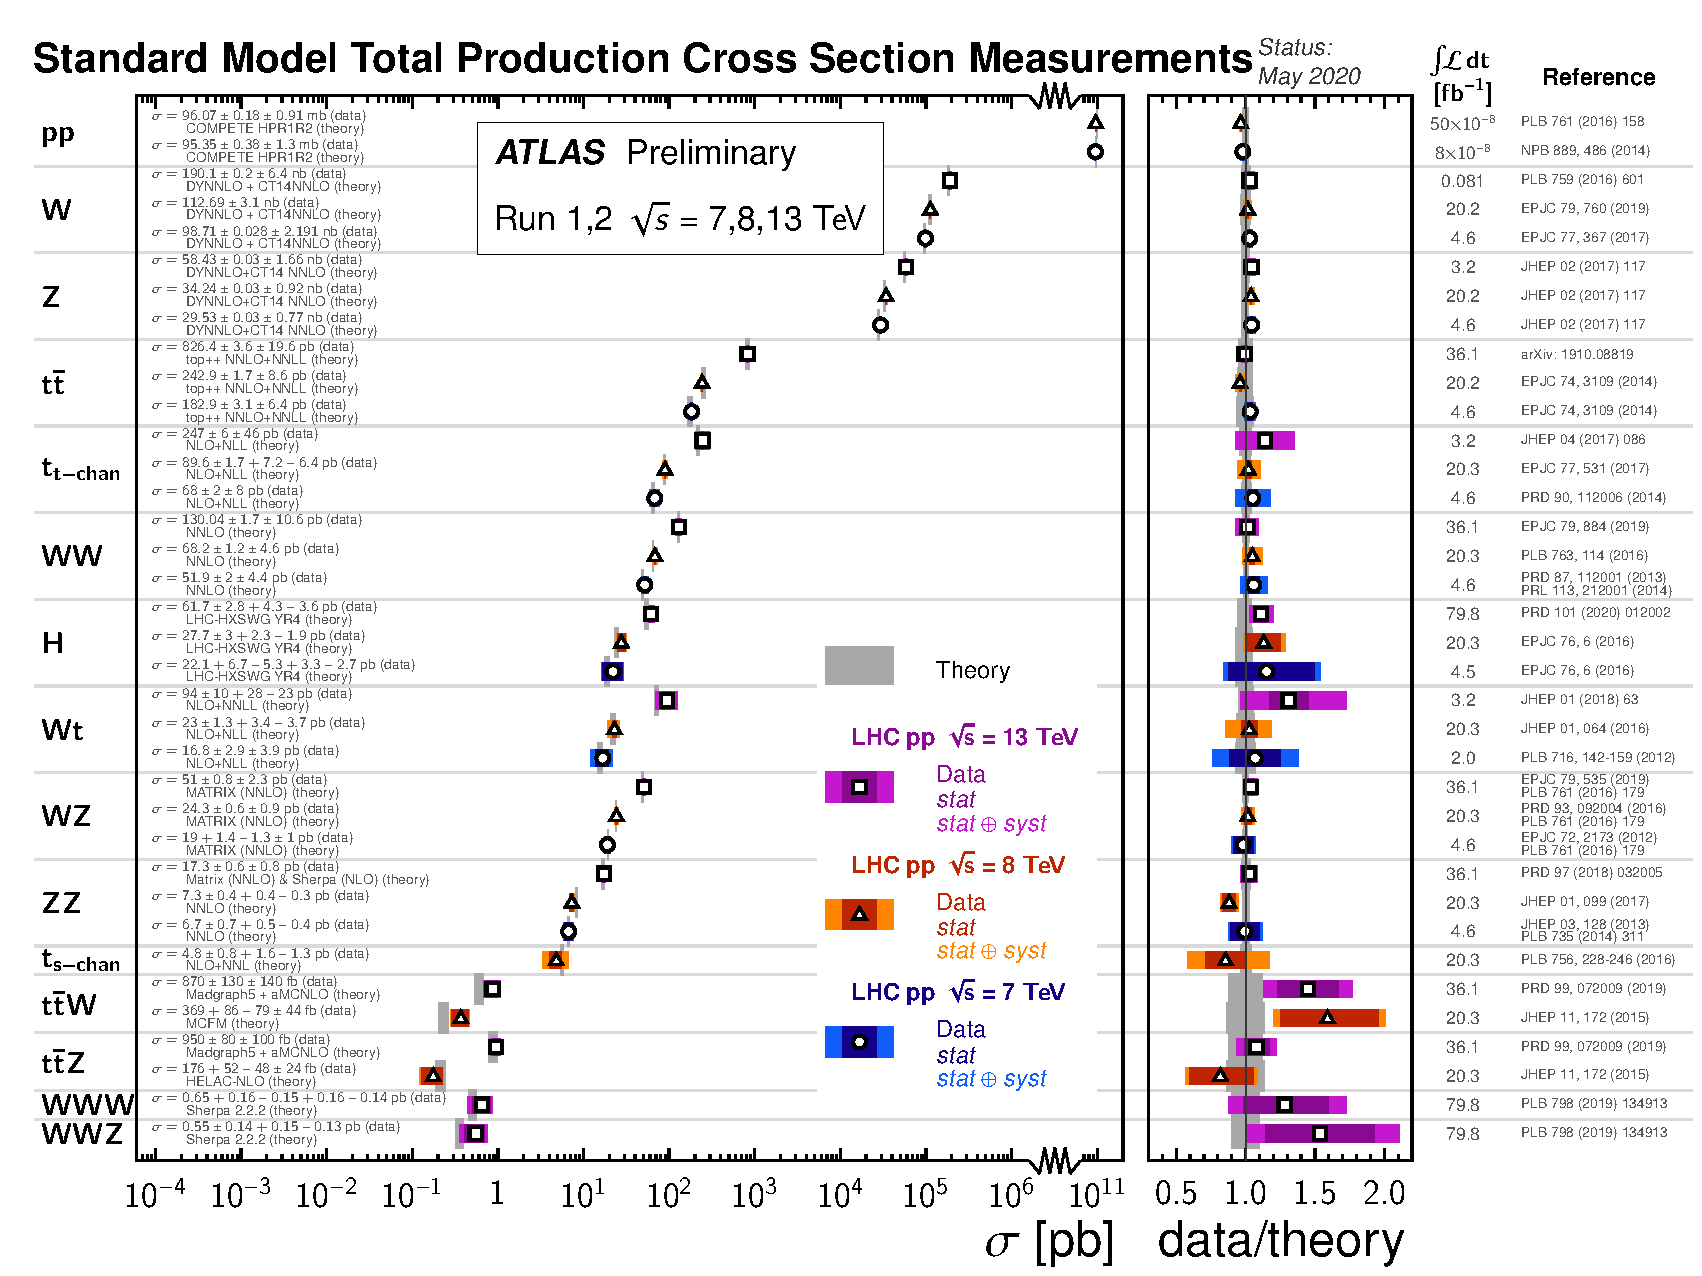
\includegraphics[width=1.05\textwidth]{figures/standardmodel/sm_processes_atlas_fig_02.pdf}
    \caption{Summary of several Standard Model total production cross-section measurements, corrected for branching fractions, compared to the corresponding theoretical expectations and ratio with respect to best theory prediction. Figure reproduced from Ref.~\cite{ATL-PHYS-PUB-2020-010}.}
    \label{fig:sm:atlas-measurement}
\end{figure}

\section{Limitations of the Standard Model}
\label{sec:sm:limitations}
Despite the SM's success in providing the most complete and solid theoretical framework to date, several observed phenomena cannot be explained by the SM. They suggest the existence of a more fundamental theory, of which the SM is the low-energy limit. This section presents a non-exhaustive account of both fundamental and aesthetic shortcomings of the SM and open questions in fundamental physics.
\begin{itemize}
    \item The SM only describes three out of the four known fundamental interactions. Gravity is most successfully described by Einstein's theory of General Relativity, which is mathematically incompatible with the formulation of the SM as a renormalisable quantum field theory~\cite{DeWitt1967,DeWitt1967-2,DeWitt1967-3,Feynman2018}. At present, this is merely a theoretical problem, as current experiments are either sensitive to quantum effects, where the minuteness of particle masses justifies neglecting gravity, or to the gravitational pull of extended objects, which do not show quantum behaviour. Eventually, a complete and consistent quantum theory of gravity is required for a truly fundamental description of Nature.
    \item In its original formulation, the SM does not account for neutrino masses. The experimental observation of neutrino flavour oscillations indicates that neutrinos have non-vanishing mass~\cite{GonzalezGarcia2008}. The mixing of the neutrino-mass eigenstates to give the weak neutrino eigenstates is described --- similarly to the CKM matrix --- by the Pontecorvo–Maki–Nakagawa–Sakata matrix~\cite{Pontecorvo1967,Maki1962}. The direct measurement of the neutrino masses and the determination of the neutrino mass hierarchy is a current object of research~\cite{Aker2020}.
    \item The vast prevalence of matter over antimatter in the universe is puzzling, as it is natural to assume that in the early universe both matter and antimatter were created in equilibrium. The violation of CP symmetry could explain the matter-antimatter asymmetry~\cite{Sakharov1991}. However, the CP violation in the SM, appearing as a complex phase in the quark mixing matrix of the weak interaction, is by far not sufficient to explain the observed asymmetry.
    \item The energy scale of electroweak symmetry breaking is \(\mathcal{O}(\SI{100}{\giga\electronvolt})\). If the SM were the fundamental theory of Nature, it would be expected to describe phenomena up to the Planck scale, defined by \(m_{\text{Planck}} = 1 / \sqrt{8 \pi G} = \mathcal{O}(\SI{e18}{\giga\electronvolt})\), where \(G\) denotes Newton's constant. The scalar Higgs boson mass receives quadratically divergent radiative loop corrections \(\Delta m_{h}\) from all particles interacting with the Higgs field. Including these corrections, the square of the Higgs boson mass is
    \begin{align}
        m_{h}^{2} = (m_{h}^{\text{bare}})^2 + \Delta m_{h}^2 = (m_{h}^{\text{bare}})^2 + \text{const.} \times \Lambda^2,
    \end{align}
    where \(\Lambda\) is the fundamental scale parameter of the theory.
    Given the measured Higgs boson mass  \(m_{h} = \SI{125}{\giga\electronvolt}\), the theory requires a precise fine-tuning of \(m_{h}^{\text{bare}}\) over more than \(10^{36}\) orders of magnitude, which is not considered to be aesthetic~\cite{Murayama2000}.
    \item Astrophysical observations strongly indicate that the baryonic matter described by the SM is insufficient to account for phenomena on scales ranging from galactic rotation curves to cosmology. An additional matter component, the so-called dark matter is required to describe the observed phenomena accurately. \Cref{sec:dm} provides a detailed discussion of the research programme defined by dark matter.
\end{itemize}
